\documentclass[11pt, a4paper]{article}

\usepackage[utf8]{inputenc}
\usepackage{geometry}
\usepackage{graphicx}
\usepackage{amsmath, amssymb}
\usepackage{caption}
\usepackage{subcaption}
\usepackage{hyperref}
\usepackage{booktabs}
% Set page margins
\geometry{left=2.5cm, right=2.5cm, top=2.5cm, bottom=2.5cm}

% Set graphics path
\graphicspath{{images/}}

\title{Supplementary Materials for "Non-Planar Hierarchical Extending Meta-Materials for Deployable Load-Bearing Structures"}
\date{}

\begin{document}

\maketitle

\section{PET Design}
The authors of this work invented the Pop-Up Extending Truss (PET) where it is first described in [1]. PETs are a novel scissor variant that flat packs when stowed and pops up into a triangular truss when deployed. 
\begin{figure}[ht]
\centering
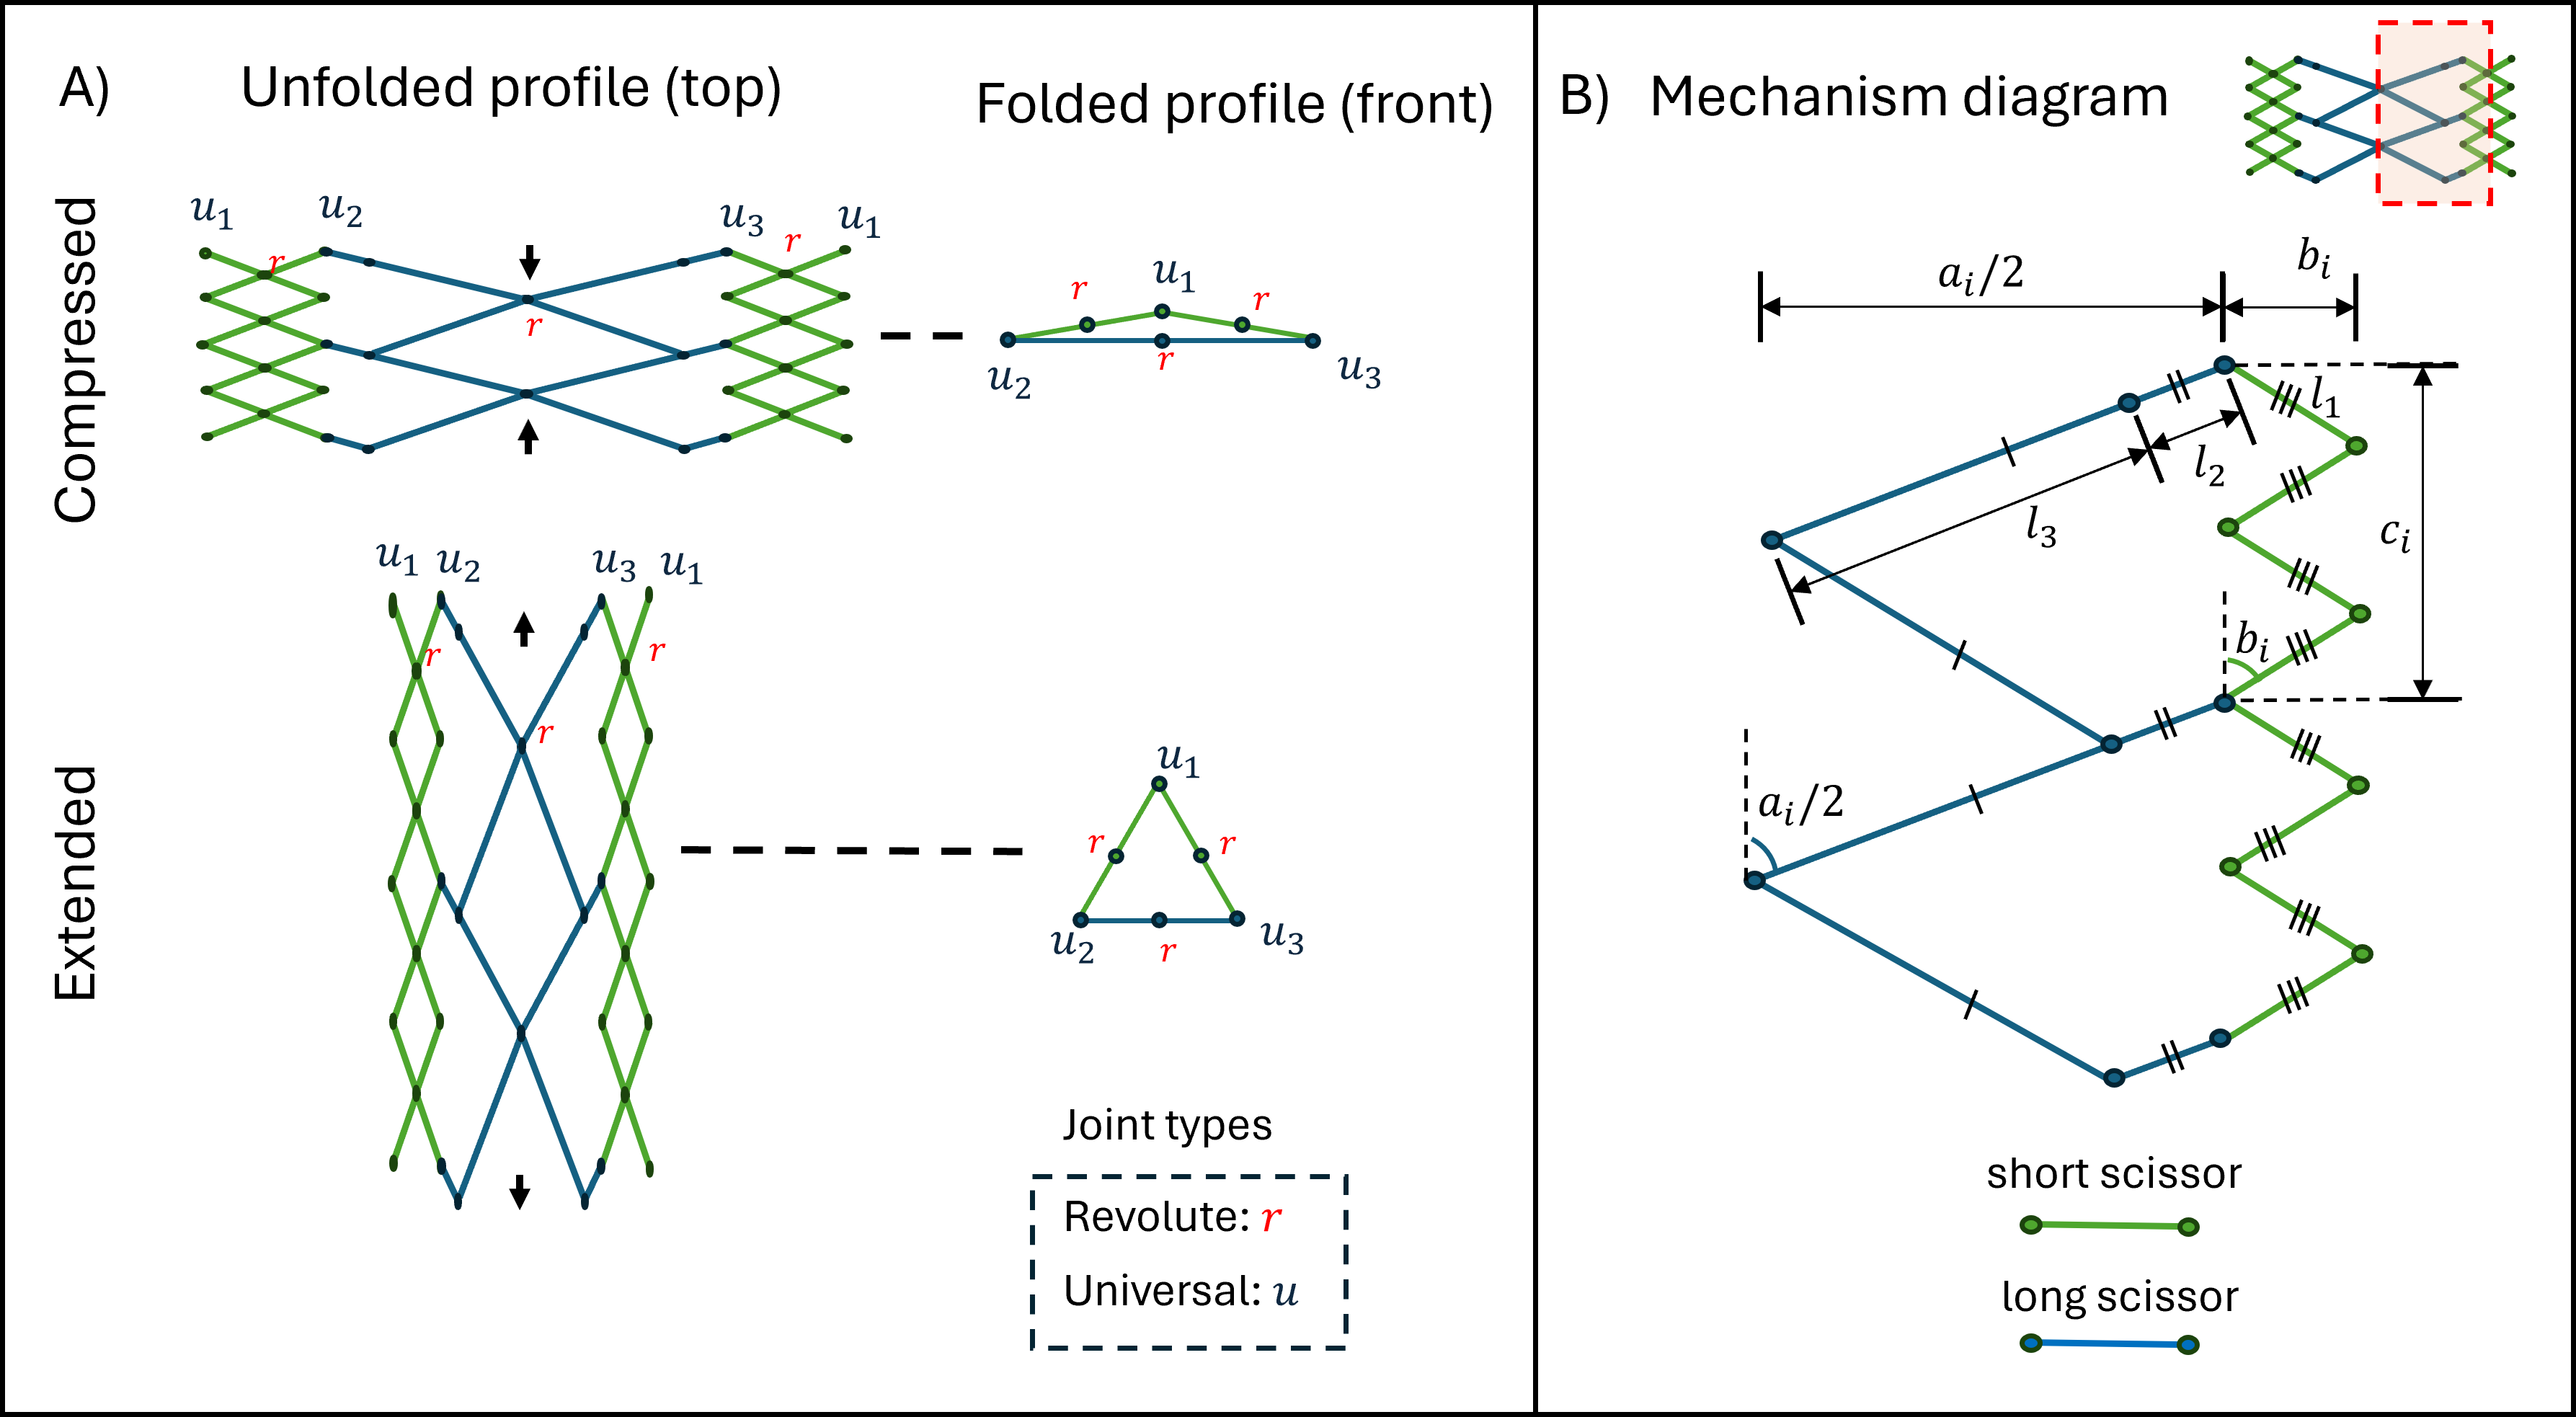
\includegraphics[width=\linewidth]{figures-sup/PET relations.png}

\centering
\caption{This figure presents the Pop-Up Extending Truss (PET) structure design parameters. A) Universal and Revolute joints can be used to construct the structure. B) Link lengths govern the properties and behavior of deployment.}
\label{fig:PET_parameters}
\end{figure}

\subsection{Design Parameters}
The Pop-up Extending Truss (PET), seen in Figure \ref{fig:PET_parameters}, which shows various unfolded views of the structure, is defined by the following parameters:
\begin{itemize}
    \item $l1 \rightarrow$ Half the length of the short-scissor member
    \item $l2 \rightarrow$ The length of the long-scissor member extension
    \item $l3 \rightarrow$ Half the length of the long-scissor member
    \item $\alpha \rightarrow$ The angle between the long-scissor members
    \item $\beta \rightarrow$ The angle between the short-scissor members
    \item $t \rightarrow$ The thickness of the square crossectional members 
\end{itemize}

\subsection{Kinematics}
To ensure that the PET is kinematically feasible, the following constraints have been formulated for any instance $i$ in the discrete deployment sequence: 
\begin{align}
    &a_i \leq 2*b_i \label{tri1}\\
    &c_i \leq l2+d1_i \label{tri2}\\
    &d1_i \leq l2+c_i \label{tri3}\\
    &d1_i^2 + d2_i^2 -c_i^2-l3^2-2*(l2*(l2+l3)) = 0 \label{eq:trap}
    % &\alpha_{i+1} \geq \alpha_i \\
    % &\beta_{i+1} \geq \beta_i \\
    % &0 \leq \alpha_{i} \leq \pi \\
    % &0 \leq \beta_{i} \leq \pi \\ %\quad \forall i \in 1:I\\
    % &l2 > 0 \\
    % &l3 > 0
\end{align}Where:
\begin{align}
    &a_i = (l2+l3)*\sqrt{(2*(1-\textrm{cos}(\alpha_i)))} \\
    &c_i = \begin{aligned}
    \sqrt{(l2 (\sin(\alpha_i/2) + \sin(3 \alpha_i/2)))^2} \\+ (2 \cos(\alpha_i/2) (l2 \cos(\alpha_i) + l3))^2 \end{aligned}\\
    % &c_i = \sqrt{(l2 (\sin(\alpha_i/2) + \sin((3 \alpha_i)/2)))^2 +} \\&\quad\quad\quad (2 \cos(\alpha_i/2) (l2 \cos(\alpha_i) + l3))^2 \\
    &\beta_i = \cos^{-1}(1-0.5(\frac{c_i}{2l1})^2) + \pi \\
    &b_i = l1 *\sqrt{(2*(1-\textrm{cos}(\beta_i)))} \\
    % &c_i = n*(l1)*\sqrt{(2*(1-\textrm{cos}(\pi-\beta_i)))}\\
    &d1_i = \sqrt{(l3^2+l2^2 - 2*(l3*l2)*\textrm{cos}(\alpha_i))} \\
    &d2_i = \begin{aligned} \sqrt{((l2+l3)^2+l3^2)\quad\quad\quad} \\- 2(l3(l2+l3))\cos(\pi-\alpha_i) \end{aligned}\\
    &\theta_i = \textrm{cos}^{-1}((a_i^2-2*b_i^2)/(-2*b_i^2))
\end{align}

\begin{figure}[ht]
\centering
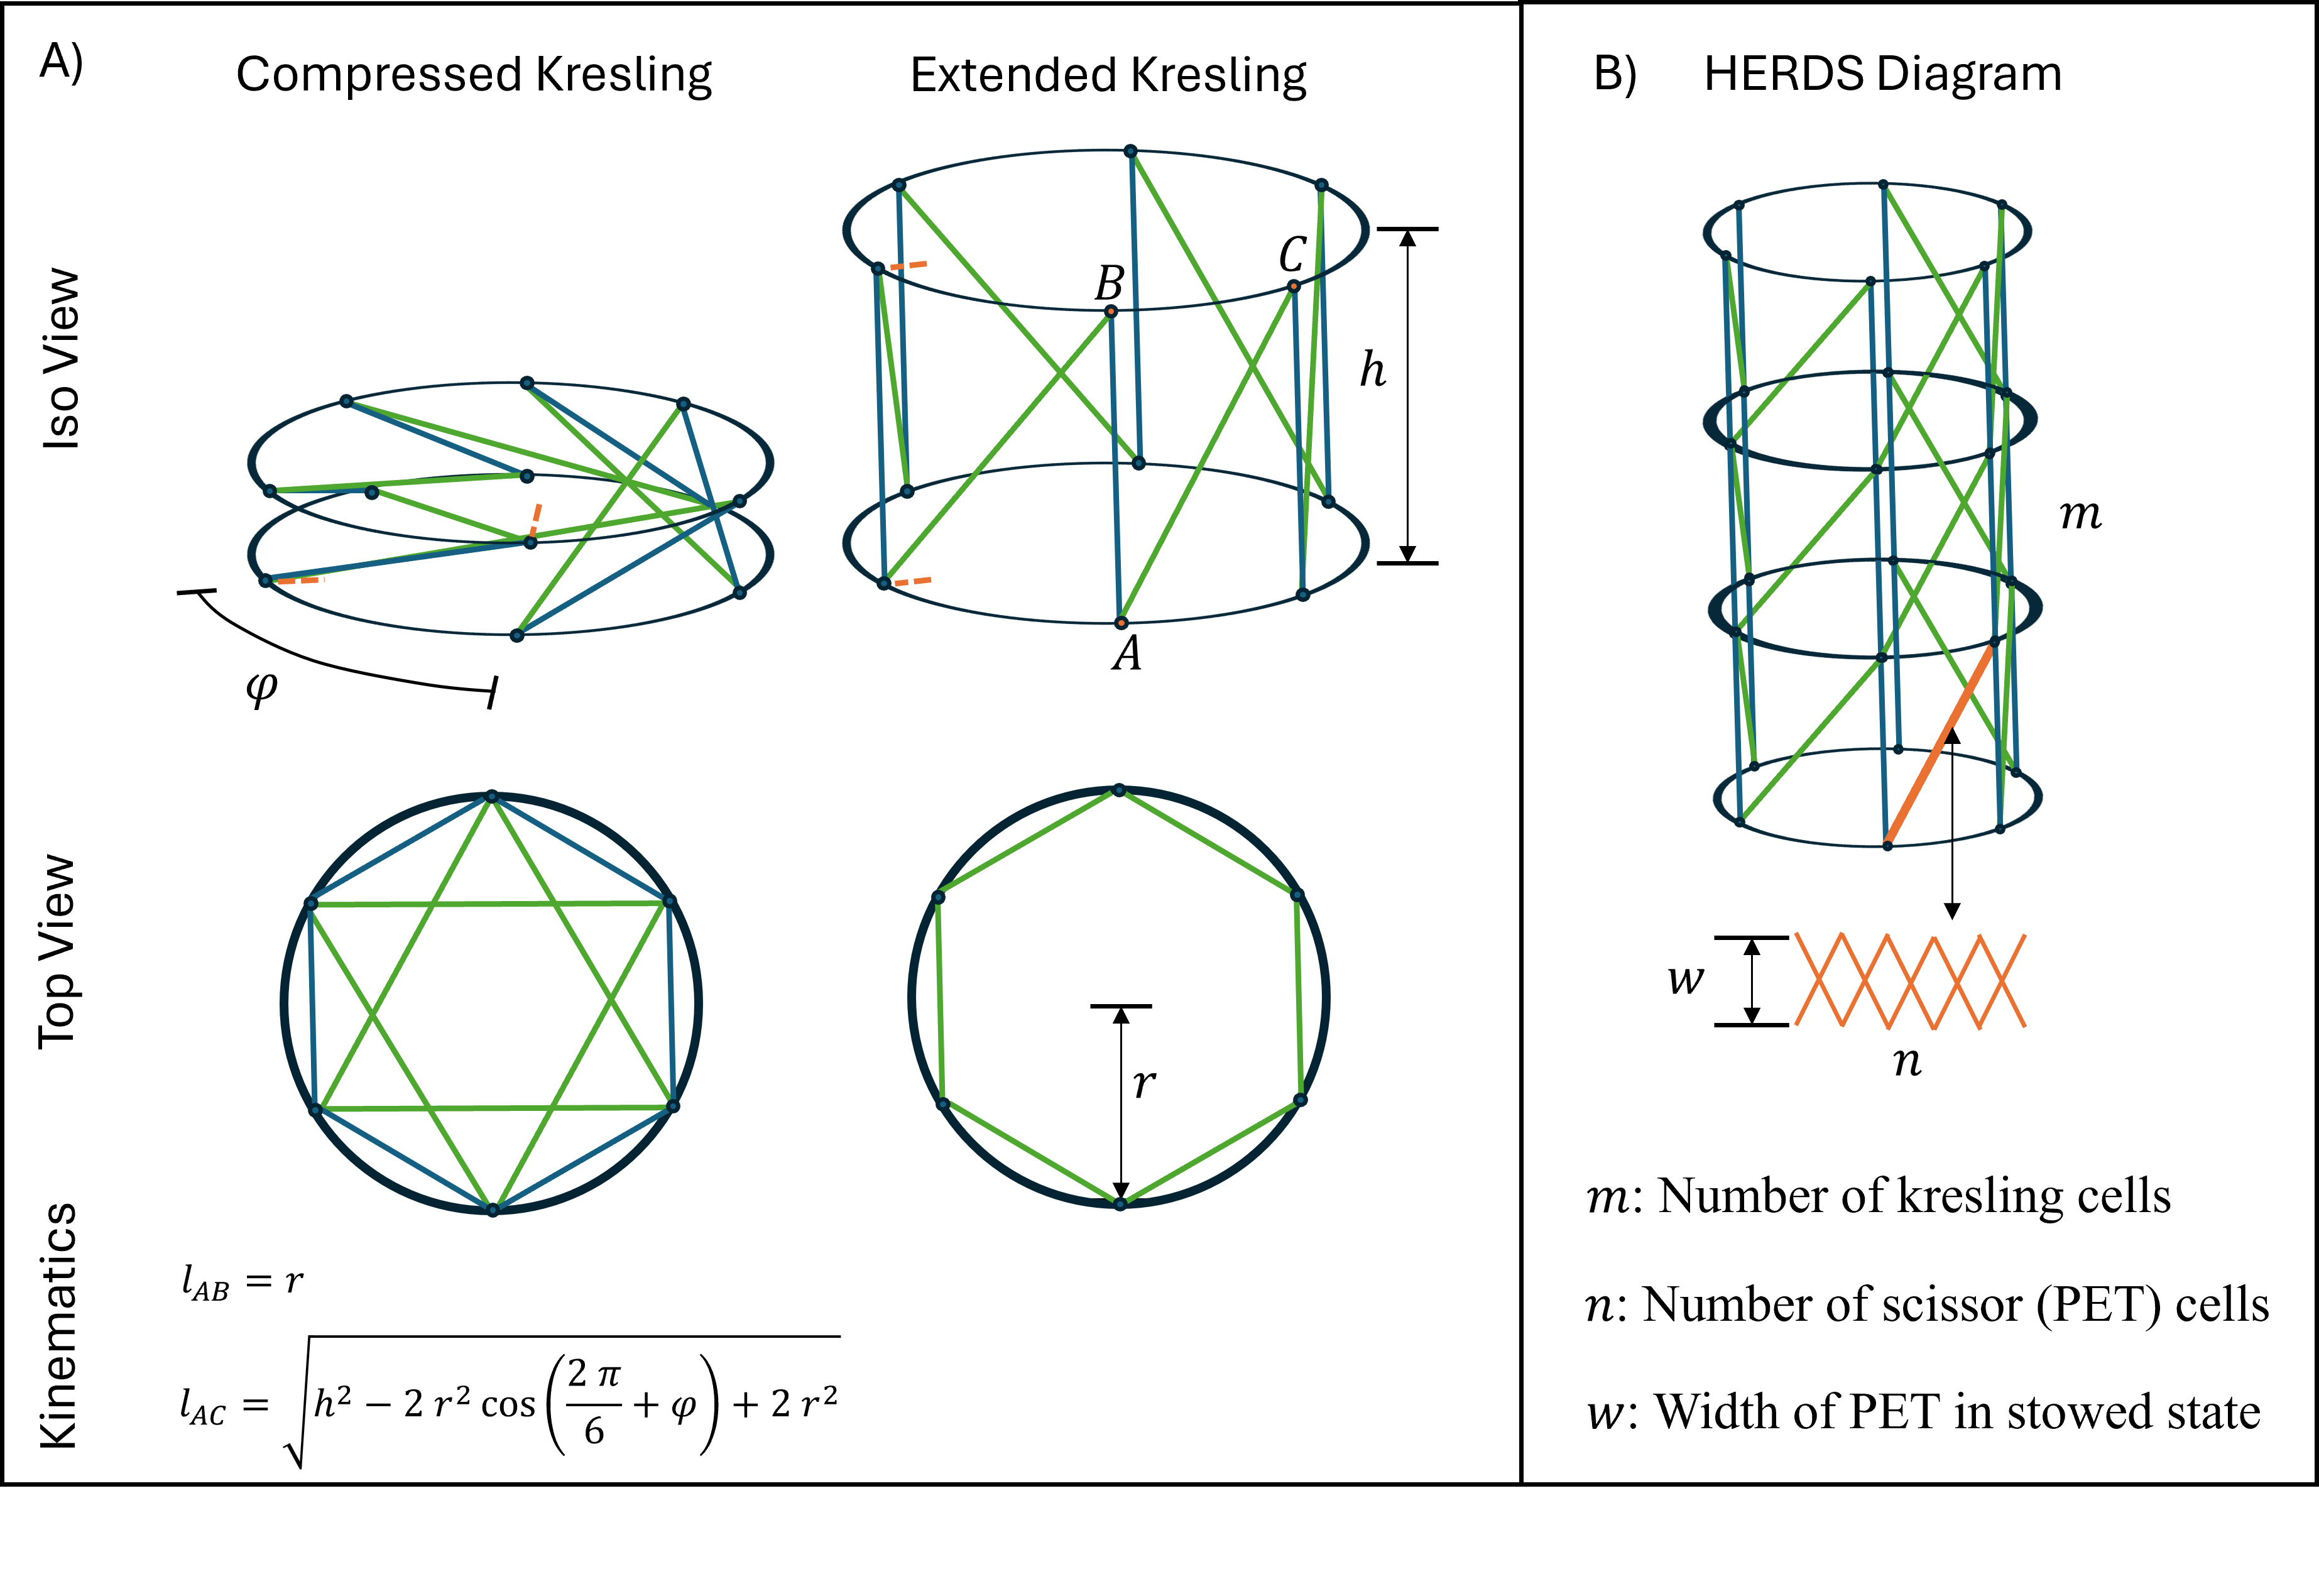
\includegraphics[width=\linewidth]{figures-sup/Kresling relations.png}

\centering
\caption{This figure presents the kresling design parameters. A) kresling deployment occurs based on the input angle $\phi$, with beam length $l_{AC}$ changing based on other parameters. B) HERDS made from PETs and Kreslings are described by the given parameters.}
\label{fig:Kres_parameters}
\end{figure}

\section{Alternative HERDS Structure Combinations}
This work discussed a hierarchically composed HERDS structure using the Kresling and PET substructures. However, various scissor variants and mechanisms could also be used as substructures for a HERDS system.  
\subsection{Scissor Variations}
There are a variety of interesting scissor variations that could be used to replace the PET scissor mechanism. Some of these include a branched scissor mechanism with three-way symmetry,  a branched scissor mechanism with four-way symmetry, as well as connecting three scissor mechanisms in a triangular configuration using uniform link lengths seen in Figure \ref{fig:tri-scissor} or using variable link lengths in Figure \ref{fig:bending HERDS}.

\begin{figure}
\centering
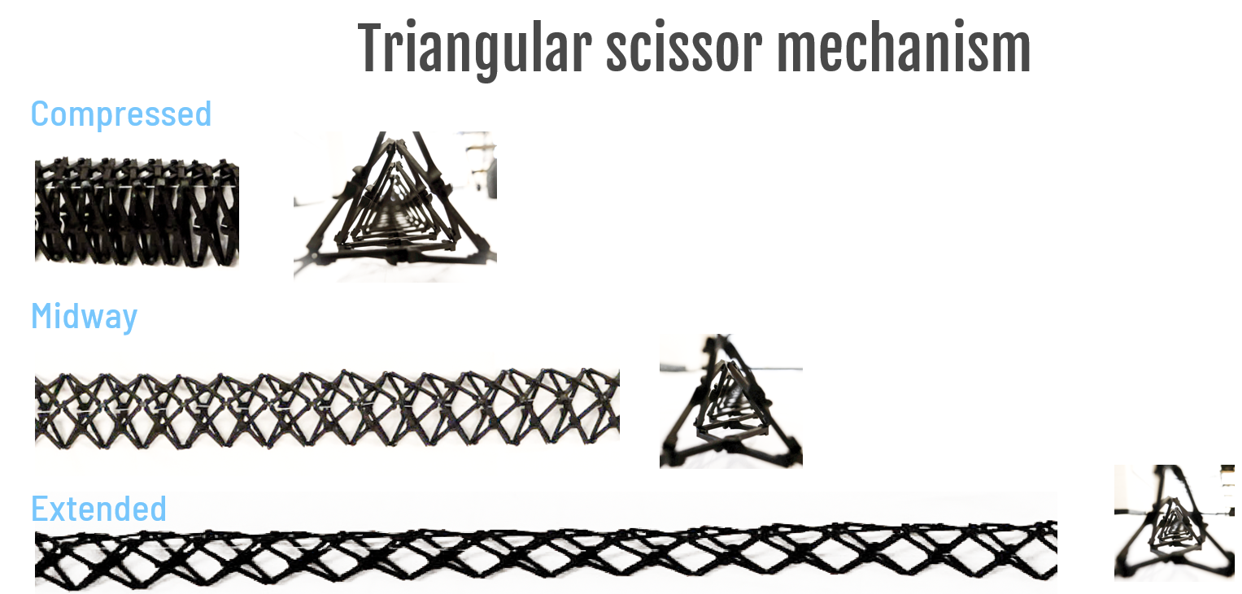
\includegraphics[width=\linewidth]{figures-sup/tri-scissor-mechanism.png}
\centering
\caption{A 3D printed prototype of a triangular scissor mechanism, an alternate substructure variant, with uniform link lengths.}
\label{fig:tri-scissor}
\end{figure}

\begin{figure}
\centering
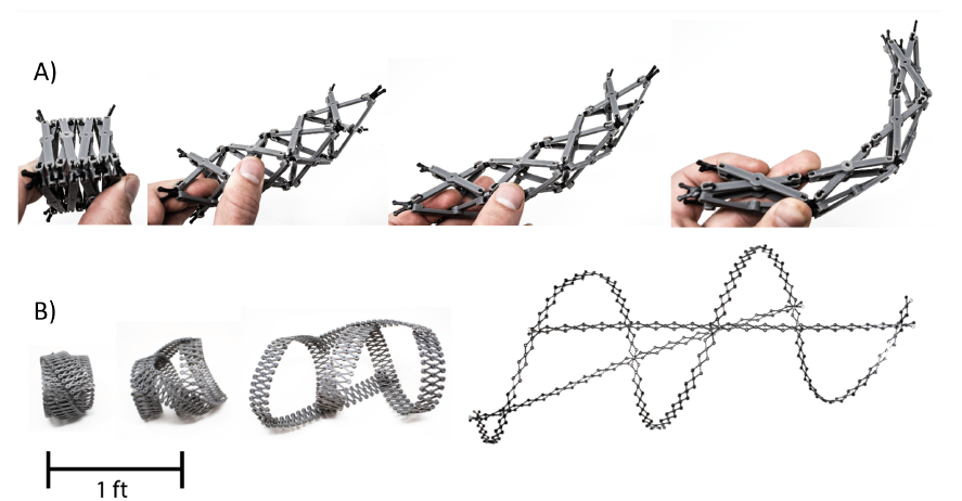
\includegraphics[width=\linewidth]{figures-sup/alternate Herd and scissor.png}
\centering
\caption{Alternate HERDS and substructure variations. A) Adjusting link lengths creates bending deployment in triangular scissor mechanisms. B) HERDS can also be created from scissor mechanisms and Handed Shearing Auxetics (HSAs).}
\label{fig:bending HERDS}
\end{figure}

\subsection{Reinforcement Strategies}
This work considered structures that can support loading, so reinforcement and locking strategies were critical to the success of the sub and superstructures. With many of the prototypes being constructed from 3D printed PLA, one way we found to extend the structural performance was by adding reinforcement cables, as seen in Figure \ref{fig:cable-reinforcing}. After the structure is deployed, it is critical to consider locking to support loads without large deformations. For this, we investigated seven locking strategies: pin and corner lock, pin lock, ramp and corner lock, and ramp lock. We also considered other nominal cases, such as no lock, glued pin, and completely rigid designs. These locks were tested using a 3-point bend test in an Instron machine, where each was tested multiple times to a 10mm deformation. The results from this test can be seen in Figure \ref{fig:locking}. The results are normalized to the rigid design, where the glued pin performed best with an 80\% effectiveness compared to rigid connections. This design is valid if the structure only needs to be deployed once. However, there are many applications where retraction is also necessary, and for that, pin and corner locks seemed to perform the best with 53\% effectiveness. It is important to note that better results could be achieved with more research and emphasis on locking, but this was out of the scope of this work. While this was not the primary consideration of this work, it is critical to the practical considerations of deployable load-bearing systems, and so we wanted to include some of our initial investigation into this aspect of the design. 


\begin{figure}
\centering
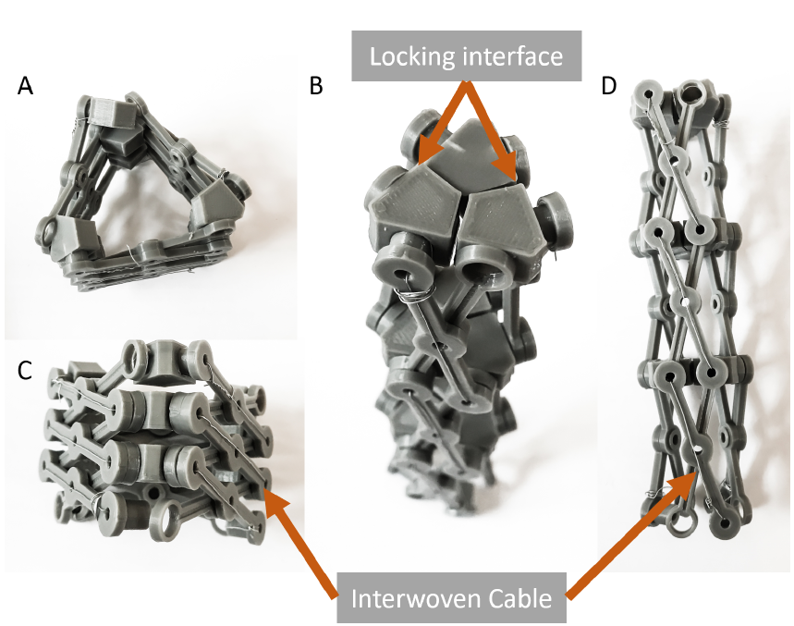
\includegraphics[width=\linewidth]{figures-sup/cable reinforced scissor.png}
\centering
\caption{HERDS, PETS, and Tri-Scissor Mechanisms can be additionally strengthened with integrated cable reinforcement.}
\label{fig:cable-reinforcing}
\end{figure}

\begin{figure}
\centering
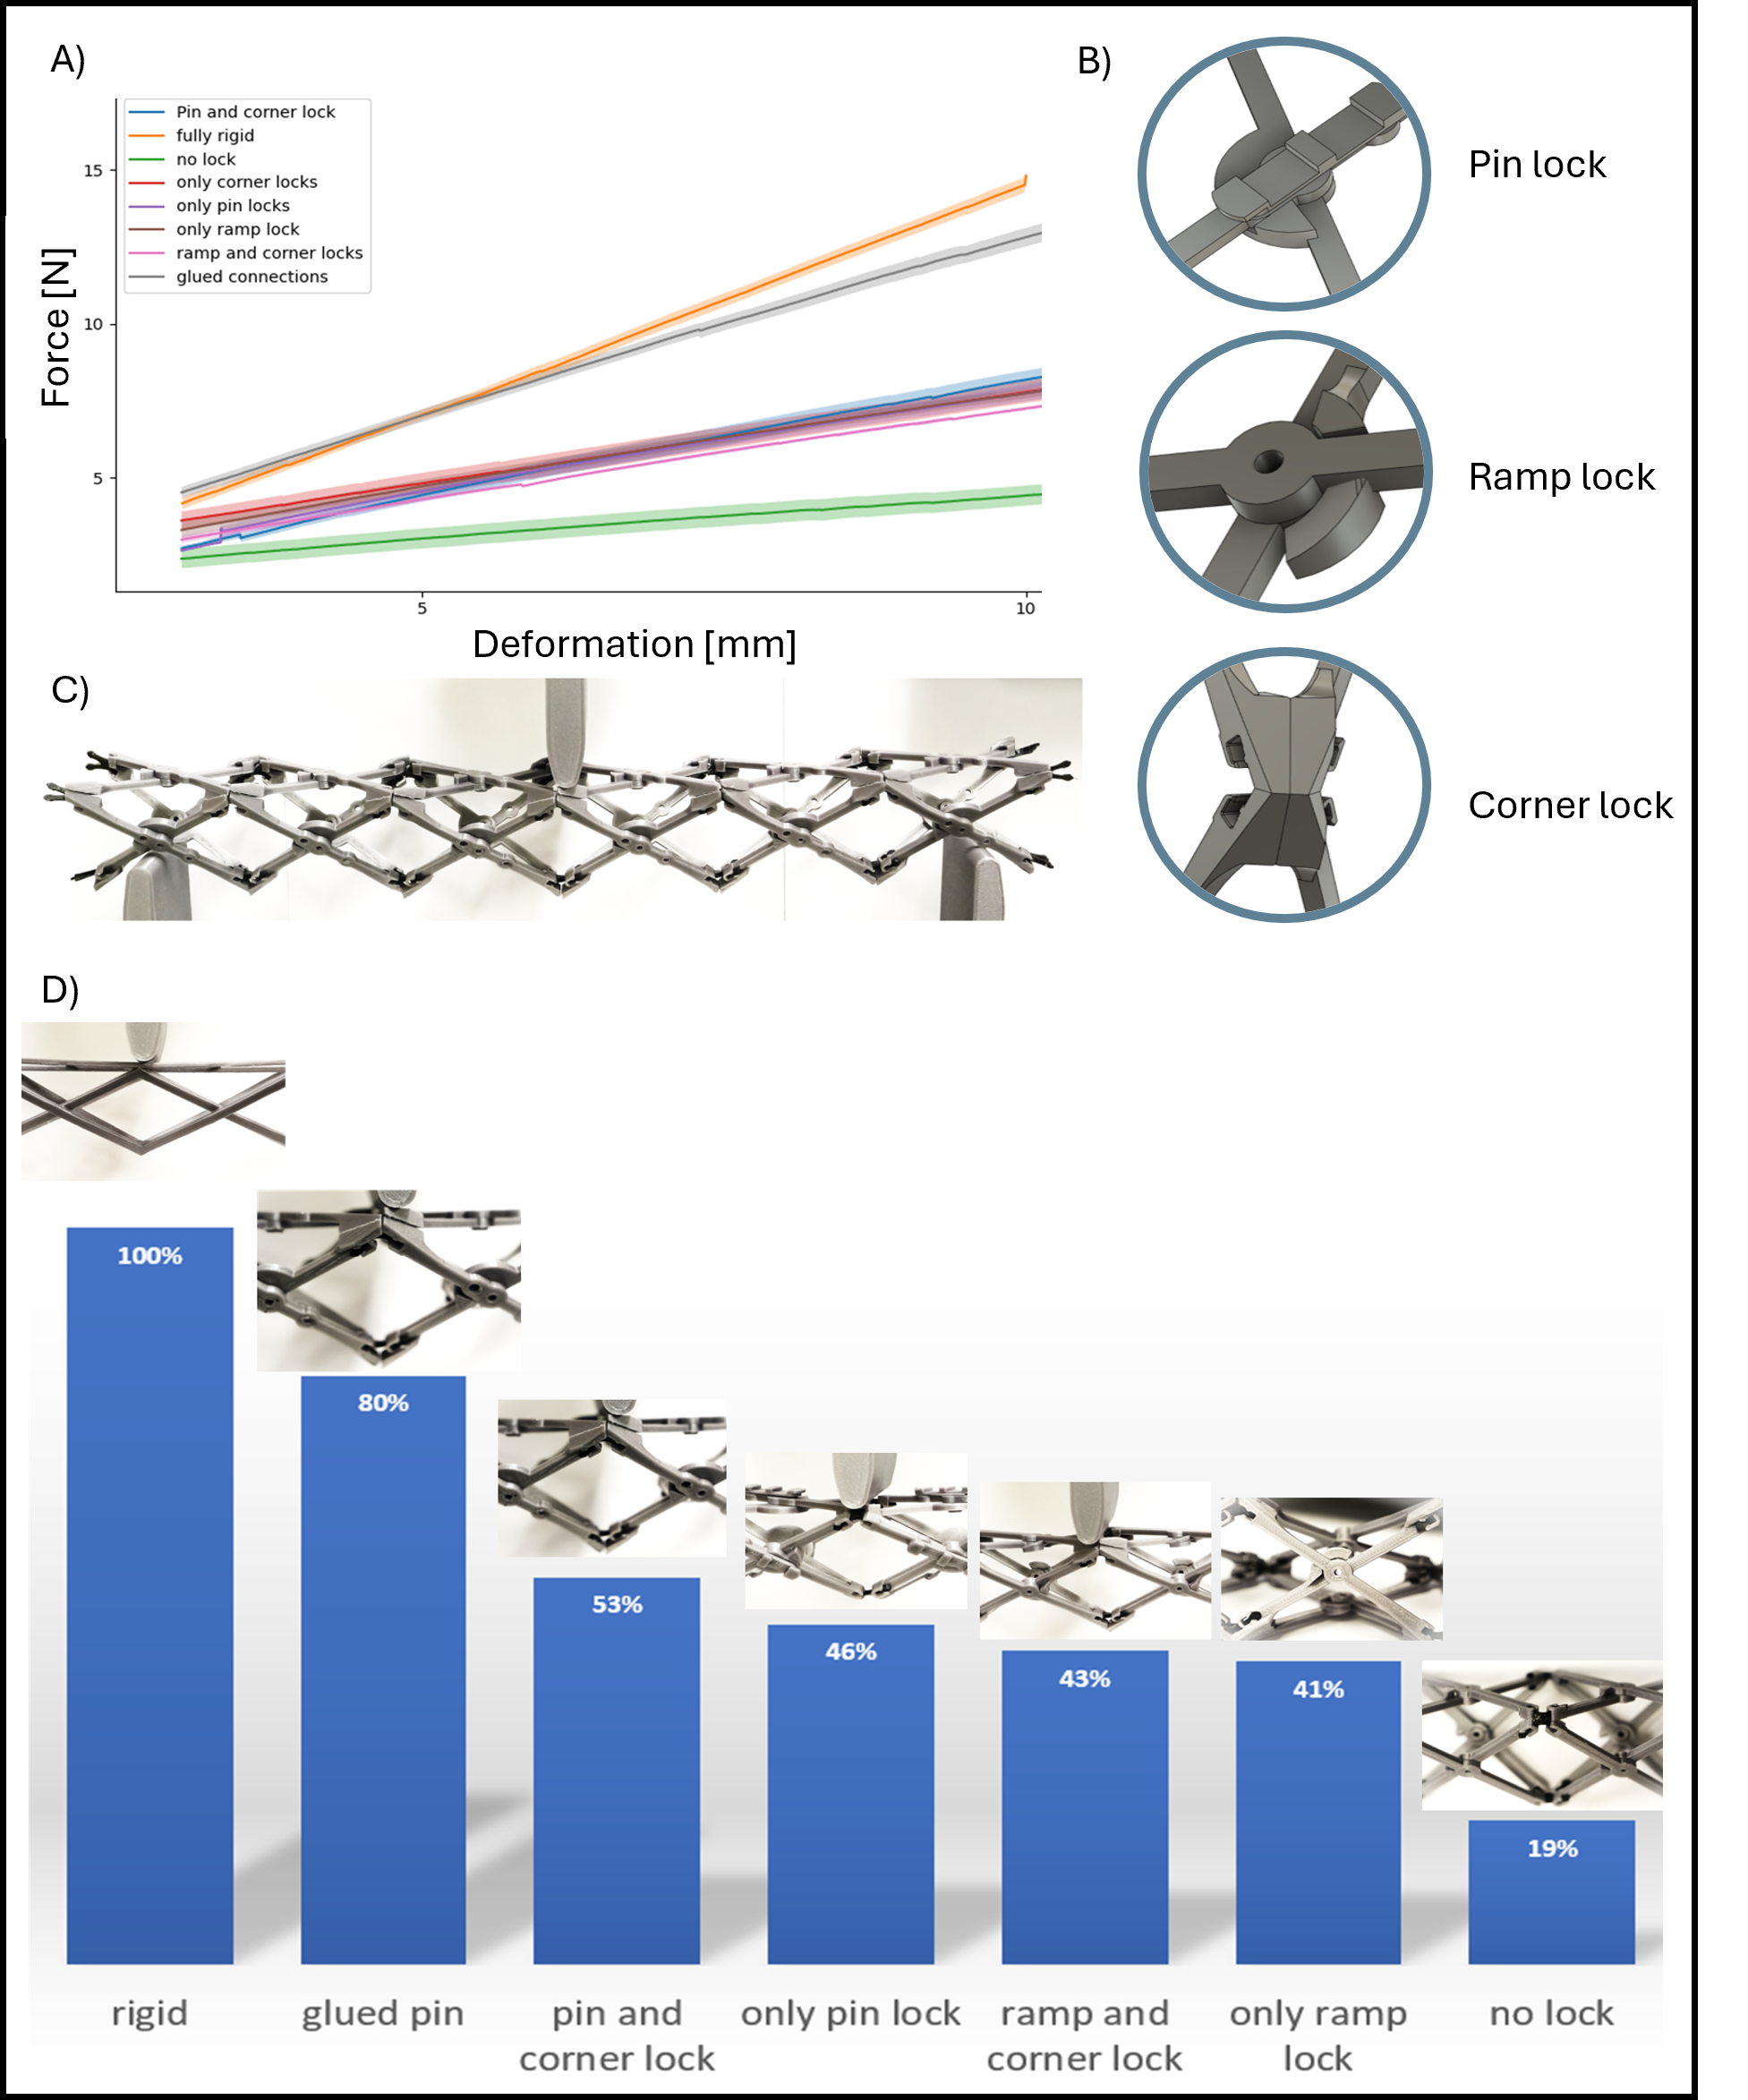
\includegraphics[width=\linewidth]{figures-sup/locking.png}

\centering
\caption{To validate various options for structure locking, we physically compared several 3D-printed lock combinations. A) Bending results based on Instron 3-point-bend physical testing. B) Diagrams of different 3D-printed lock variations. C) Stiffness comparison of physical test results.}
\label{fig:locking}
\end{figure}

\section{Kresling Design}
The Kresling was the other substructure used for the hierarchical composition of the extending mechanism. The mechanical Kresling, as opposed to the very common origami version, was described by Zhai et al. [56]. In this section, we provide more information about this structure's design parameters and kinematics seen in Figure \ref{fig:Kres_parameters}. 
\subsection{Design Parameters}
The following parameters define the Kresling mechanism:
\begin{itemize}
    \item $r \rightarrow$ The radius of the structure
    \item $\phi \rightarrow$ The twist angle between the top and bottom plates
    \item $h \rightarrow$ The height between the top and bottom plates
\end{itemize}
\subsection{Kinematics}
To make sure that the structure is kinematically feasible, the member lengths have to be supported by the following equations:
\begin{align}
    &l_{AB} = r\\
    &l_{BC} = \sqrt{h^2-2r^2\textrm{cos}(\phi)+2r^2} \\
    &l_{AC} = \sqrt{h^2-2r^2\textrm{cos}(\frac{2\pi}{6}+\phi)+2r^2}
\end{align}

\section{HERDs Design}
This section details specific parameters for the hierarchically composed structure that uses the Kresling and the PET as substructures. 
\subsection{Design Parameters}
In addition to the PET and Kresling design parameters, the HERDS superstructure also has various parameters as follows:
\begin{itemize}
    \item $w \rightarrow$ The width of the PETs in the stowed state
    \item $n \rightarrow$ The number of scissor (PET) units
    \item $m \rightarrow$ The number of kresling units
\end{itemize}

\subsection{Kinematics}
The kinematics of the HERDS follow the same equations from the Kresling to ensure the state is feasible. 

\section{Ansys APDL}
\subsection{Line Body Appoximation}
We represent all models as simplified beam elements with fixed constraints between lines. The beam elements in ANSYS APDL are based on Timeshanko beam theory, which reduces the degrees of the whole solid to 6, translations, and rotations in x,y, and z. Warping is an additional degree of freedom that could be considered, but it was found to reduce the accuracy between Real2Sim data. Each line is split into elements to increase the accuracy of the deformation. The cross-section of the beam elements was assumed to be rectangular, and the cross-sectional elements can also be subdivided for better accuracy. We found diminishing returns for many line body and cross-section elements; the computational time increased, but the solution accuracy stayed constant. We used line bodies because they are more scalable than solid body meshing for our long, slender structures and provide fewer artifacts due to poorly formed meshes, leading to the joints' artificial stiffness. 

\subsection{Physical Testing Validation}
We evaluated physical bending, compression, tension, and torsion models in an Instron machine to ensure our simulation models were accurate. We printed an ASTM test specimen, a PET, a small-member scissor, and a long-member scissor in an SLA printer. We found the Youngs modulus from the test specimen which was then used for future simulation experimentation. We then tested all the models at least 5 times for each boundary condition. These boundary conditions were then evaluated for solid body and line body FEM simulations to ensure a reasonable agreement between the Real2Sim. These results can be seen in Figure \ref{fig:physical validation}.

\begin{figure}
\centering
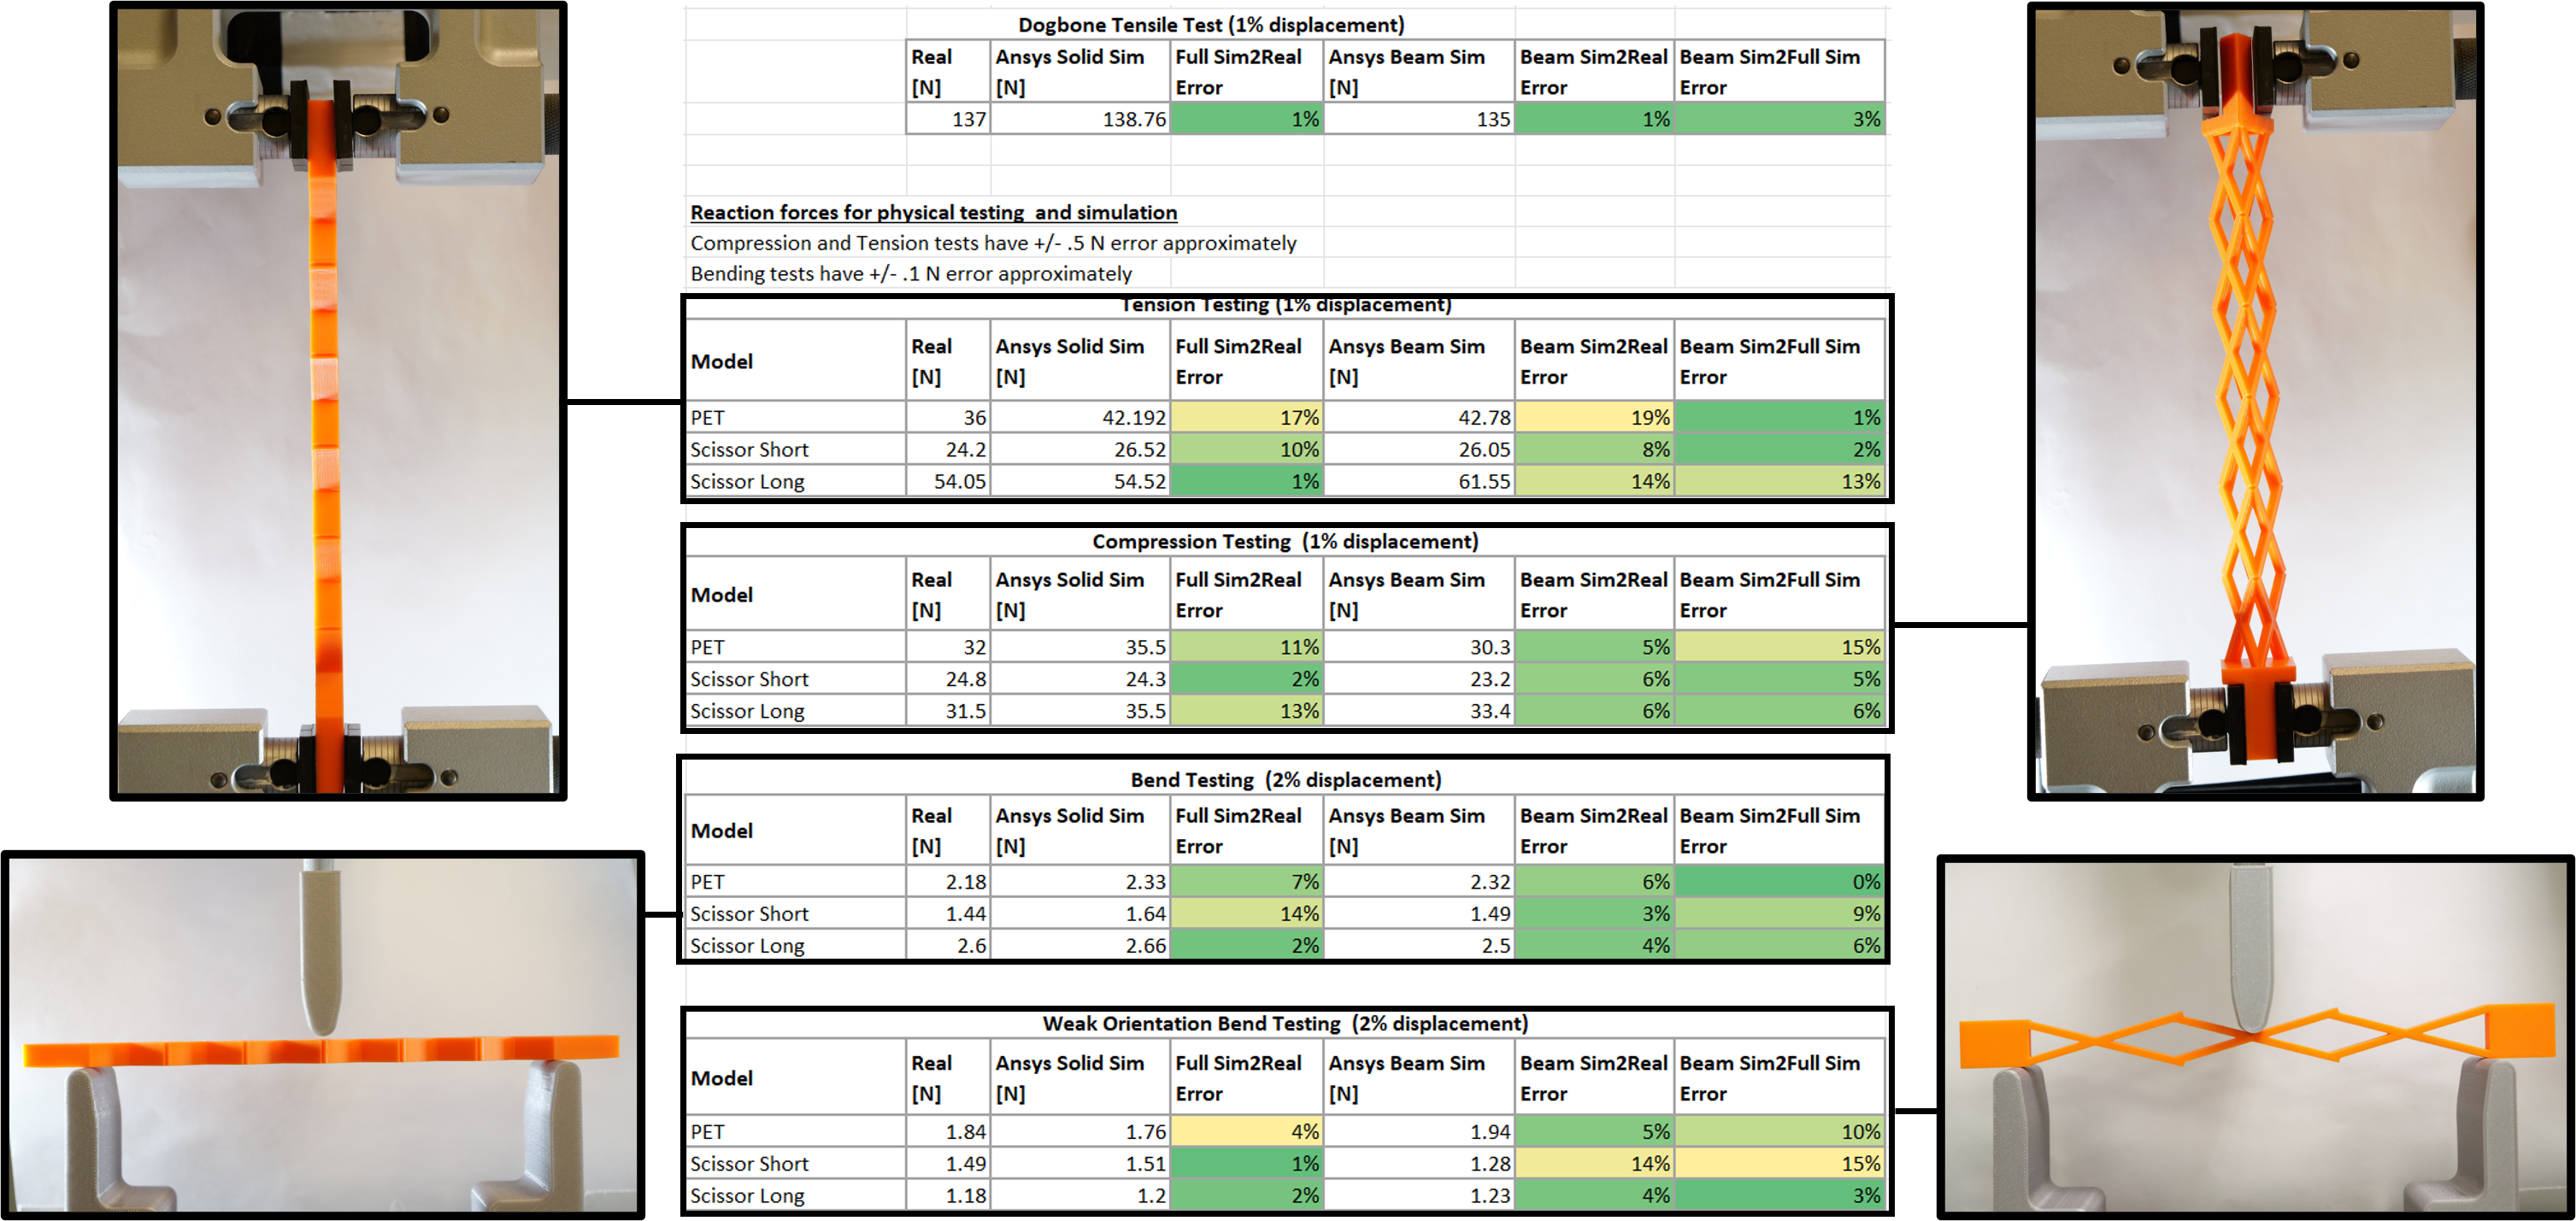
\includegraphics[width=\linewidth]{figures-sup/sim_validation.png}

\centering
\caption{We see close agreement between physical testing and simulaiton.}
\label{fig:physical validation}
\end{figure}

\subsection{Boundary Conditions}
We considered a one percent displacement in a cantilever beam, compressive, tensile, and torsional to estimate the flexural modulus and effective stiffnesses, seen in Figure \ref{fig:boundary_cond}. We chose a cantilevered beam instead of a 3-point bend because the boundary conditions represented in APDL are easier to define than a 3-point bend test on the beam elements. 

\begin{figure}
    \centering
    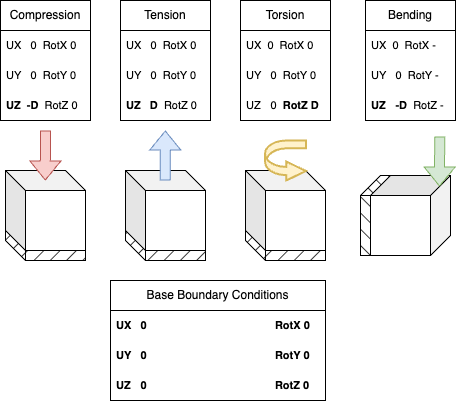
\includegraphics[width=0.75\linewidth]{figures-sup/Supplementary - Boundary Conditions.drawio.png}
    \caption{Ansys APDL boundary conditions for this study's compression, tensile, torsional, and bending tests on the PET, Kresling and HERDS structures.}
    \label{fig:boundary_cond}
\end{figure}

\subsection{Computational Considerations}
We ran the models on a local workstation running the AMD Threadripper and the Pittsburgh Supercomputer with system specifications defined in Table \ref{tb:computer}. The HERDS models with a large number of beam elements took up $>$32GB of RAM when solving the boundary condition equations and could not be solved on the Local Workstation.

% Please add the following required packages to your document preamble:
% \usepackage{booktabs}
\begin{table}[]
\centering
\caption{LOCAL WORKSTATION AND PITTSBURGH SUPER COMPUTER CONFIGURATION}
\begin{tabular}{@{}lll@{}}
\toprule
        & Local Workstation                    & Pittsburgh Super Computer                                                                                                 \\ \midrule
CPU     & \begin{tabular}[c]{@{}l@{}}AMD Threadriper\\ 16 cores, 32 threads\\ 4.5 GHz\end{tabular} & \begin{tabular}[c]{@{}l@{}}2 AMD EPYC 7742 CPUs \\ 64 cores per CPU, 128 cores per node \\ 2.25-3.40 GHz\end{tabular} \\
RAM     & 32 GB                                & 256GB                                                                                                                     \\
Storage & 500 GB NVMe SSD                      & 3.84TB NVMe SSD                                                                                                           \\ \bottomrule
\end{tabular}
\label{tb:computer}
\end{table}

\section{Design Sweep and Analysis}
We sought to sweep potential design variation and varied the designs between 5 and 200x extension ratio. For the PET this was achieved by varying the final deployment angle $\alpha$ and the member thickness. The Kresling achieved this by varying the final deployment angle $\phi$ and the member thickness. Finally, the HERDS is swept over the member thickness and PET width of "offset," correlated to the number of PET units. 

\begin{figure}
    \centering
    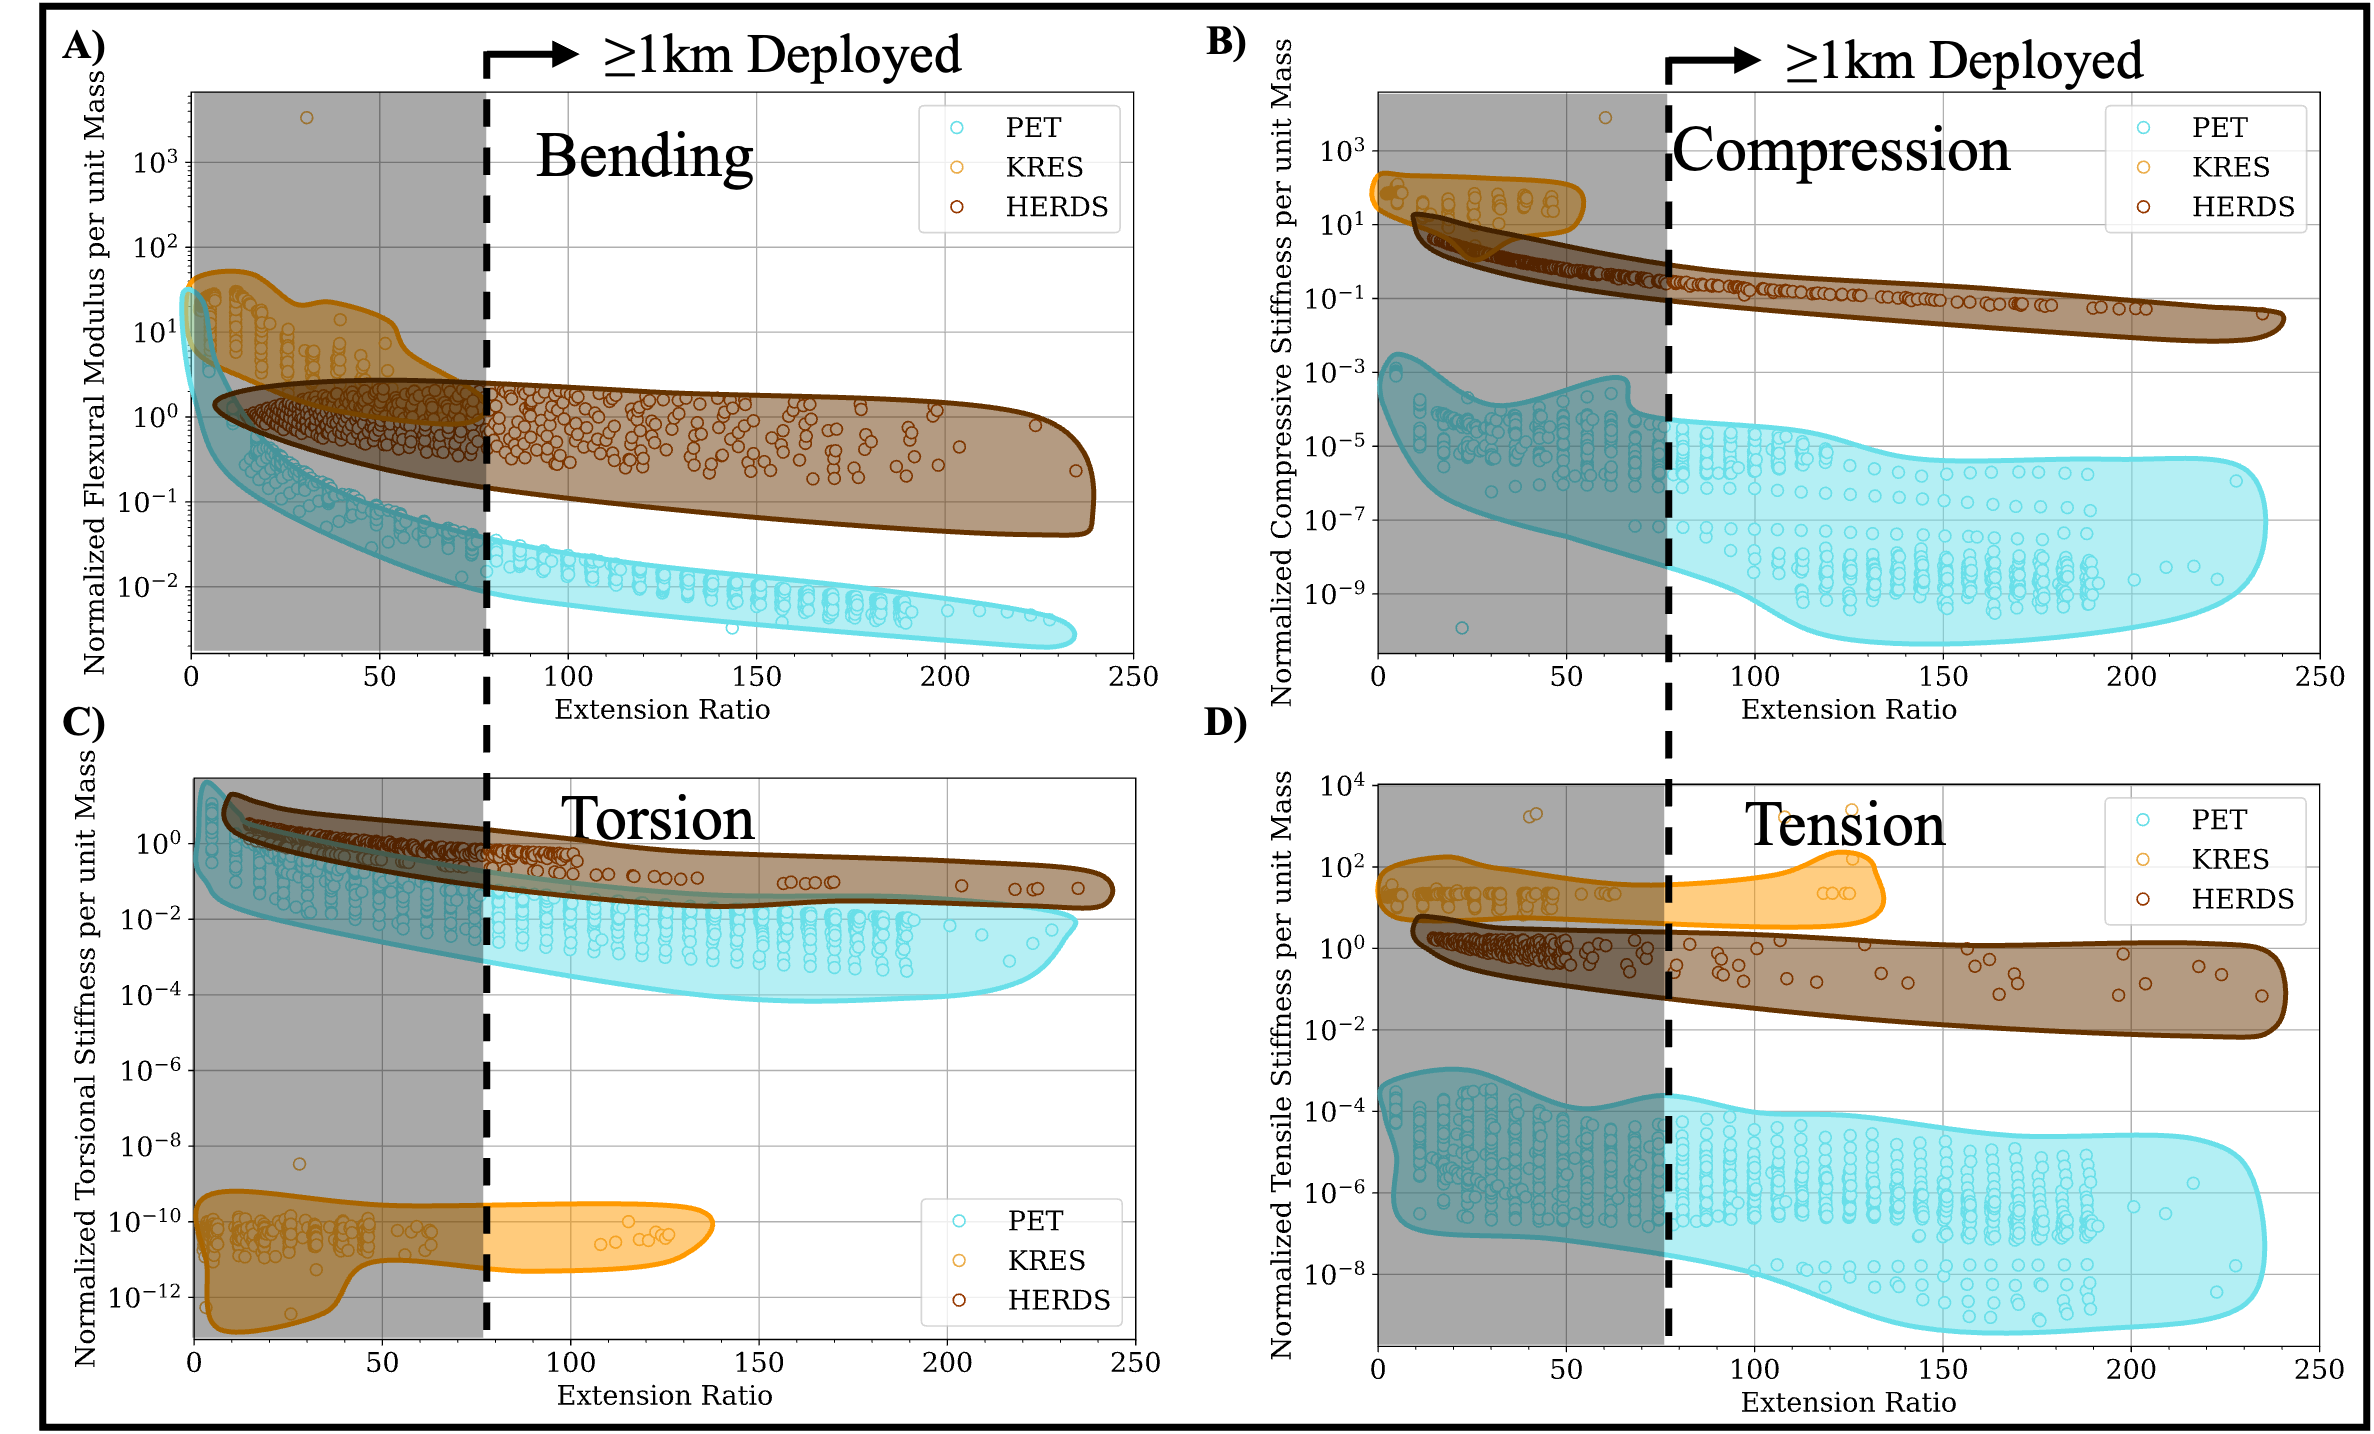
\includegraphics[width=\linewidth]{Figures/Rebuttal/fig6_sup_rebuttal.png}
    \caption{The results from the design sweep with the values normalized by the mass of the structures.}
    \label{fig:norm_mass}
\end{figure}

\begin{table}[]
\centering
\caption{DESIGN SWEEP PARAMETERS FOR PET, KRESLING AND HERDS}
\begin{tabular}{@{}lllll@{}}
\toprule
         & Extension Ratio & Deployment Angle  [rad]& Member Thickness [mm]& Offset [mm]\\ \midrule
PET      & 5$\rightarrow$200x          &                  0.52$\rightarrow$1.47&                  1.0$\rightarrow$31.4& -      \\
Kresling & 5$\rightarrow$200x          &                  $\frac{\pi}{6} \rightarrow$$-\frac{\pi}{6}$&      0.6$\rightarrow$21.9& -      \\
HERDS    & $\sim$5$\rightarrow$200x    &                  -&                  1.0$\rightarrow$10.0&        6.0$\rightarrow$50.0\\ \bottomrule
\end{tabular}
\end{table}

\begin{table}[ht]
\centering
\caption{NUMBER OF DESIGNS THAT WERE TESTED FOR EACH BOUNDARY CONDITION}
\begin{tabular}{lcccc}
\toprule
 & Bending & Compression & Tension & Torsion \\
\midrule
HERDS & 496 & 390 & 270 & 405 \\
Kresling & 813 & 289 & 343 & 363 \\
PETs & 1000 & 980 & 979 & 977 \\
\bottomrule
\end{tabular}

\label{tab:file_counts}
\end{table}
\section{Prototype Fabrication and Testing}
The HERDS prototypes were assembled using 3D-printed parts, laser-cut acrylic, and metal fasteners. Elements like joint design and locking mechanisms are crucial for the system’s functionality, requiring further refinement for targeted applications. These initial models provide a solid proof of concept and set the stage for more polished future versions. The design specifications for each prototype are detailed in Table \ref{tb:proto-config-params}.

We performed a deployment test, a compression test, and a three-point bending test in a motion capture system. Markers on the middle and top plates tracked the plates' position during deployment and measured position and deflection during experiments. 

A cable was secured to the top plate of the HERDS to evaluate deployment empirically. The bottom plate of the HERDS was free, and the structure was extended solely by the cable's tension and gravity. This demonstrated the feasibility of smooth deployment without jamming or locking. The deployment of the prototype, consisting of more than 1,500 constituent 3D printed parts, had no instances of jamming and achieved unified extension. In the stowed state it packed to a height of 5 cm and extended to a final length of approximately 254 cm.   

Weights were added to a testing setup to test the compressive capabilities of the structure. The motion capture system measured the deformation between the cell plates as weight was incrementally added. The prototype supported 65 N before failure. Plastic deformation of the 3D-printed material at the joint interface between the PET and the kresling was observed at failure. This PLA plastic prototype is not optimized for structural stiffness but highlights the significant advantage over a tethered system that could not support compressive loads. 

A tangential loading condition was evaluated on the prototype as well. Due to size and space constraints, an inverted 3-point bend test was performed. The two ends of the HERDS beam were free-standing on the ground, and the middle of the structure was lifted to apply a force. Similarly, the failure was due to plastic deformation at the joint interface between the Kresling and PET. Additional joint design with improved locking capabilities is required for future iterations. Despite these unexpected deformation modes, the model still supported up to 60 N force before failure. Improved locking, tolerances, and base material properties may enhance stiffness and offer enhanced capabilities over tethers. 

\begin{table}
\caption{\bf Hardware Prototype Parameters}
\centering
\renewcommand{\arraystretch}{1.4}
\setlength{\tabcolsep}{10pt}
\begin{tabular}{cc}
\hline
& \begin{tabular}[c]{@{}c@{}}Large \\ HERDS\end{tabular}   \\\hline
% l1                       & 0.022   & 0.022   \\
% l2                       & 0.153   & -   \\
% l3                       & 0.226   & -  \\
Thickness                        & 0.006   \\
% $\alpha_1$               & \textcolor{red}{todo}   & -        & 2.352  \\
% $\beta_1$                & \textcolor{red}{todo}   & 2.844    & 2.524  \\
PET Cells                        & 13      \\ 
% ra                        & 0.289   & 0.149  \\
% $\phi_1$                 & \textcolor{red}{todo}   & 1.046    & - \\

Kresling Cells                       & 2     \\ 
Diameter                       & 0.578    \\
% Initial Height                    & 0.024   & 0.044 \\

Initial Height                    & 0.050    \\
Final Height                    & 2.540   \\ \hline
\begin{tabular}[c]{@{}c@{}}Expansion \\ Ratio\end{tabular}        & \textbf{50.8}  \\ \hline

\end{tabular}
\label{tb:proto-config-params}
\end{table}

\bibliography{FOLDING_NAT_COM}

\end{document}
